\newpage
\section*{Part D: Exercise 7.2}

%---------------------------------------------------------------
\subsection*{Exercise 7.2, Question 1}
\textbf{Question.} Find the coordinates of the point which divides the join of $(-1,7)$ and $(4,-3)$ in the ratio $2:3$.

\textbf{Solution.} Let $A(-1,7)$, $B(4,-3)$ and $P(x,y)$ divide $AB$ internally in the ratio $m_1:m_2=2:3$. So $(x_1,y_1)=(-1,7)$, $(x_2,y_2)=(4,-3)$, $m_1=2$, $m_2=3$.

By the section formula $\left(\dfrac{m_1x_2+m_2x_1}{m_1+m_2},\dfrac{m_1y_2+m_2y_1}{m_1+m_2}\right)$:
\begin{align*}
x&=\frac{2(4)+3(-1)}{2+3}=\frac{8-3}{5}=\frac{5}{5}=1\\
y&=\frac{2(-3)+3(7)}{2+3}=\frac{-6+21}{5}=\frac{15}{5}=3
\end{align*}
\slip{$m_1$ goes with the far point $B$ ($x_2$, $y_2$) and $m_2$ with $A$ ($x_1$, $y_1$). Writing $2(-1)+3(4)$ instead would divide in the ratio $3:2$.}

\ans{The required point is $(1,3)$.}

%---------------------------------------------------------------
\subsection*{Exercise 7.2, Question 2}
\textbf{Question.} Find the coordinates of the points of trisection of the line segment joining $(4,-1)$ and $(-2,-3)$.

\textbf{Solution.} Let $A(4,-1)$, $B(-2,-3)$. The points of trisection $P$ and $Q$ divide $AB$ into three equal parts, with $P$ nearer to $A$. So $P$ divides $AB$ in the ratio $1:2$ and $Q$ in the ratio $2:1$.

By the section formula $\left(\dfrac{m_1x_2+m_2x_1}{m_1+m_2},\dfrac{m_1y_2+m_2y_1}{m_1+m_2}\right)$ with $(x_1,y_1)=(4,-1)$, $(x_2,y_2)=(-2,-3)$:

For $P$ with $m_1:m_2=1:2$:
\[
x=\frac{1(-2)+2(4)}{1+2}=\frac{-2+8}{3}=\frac63=2,\qquad y=\frac{1(-3)+2(-1)}{1+2}=\frac{-3-2}{3}=-\frac53 .
\]
For $Q$ with $m_1:m_2=2:1$:
\[
x=\frac{2(-2)+1(4)}{2+1}=\frac{-4+4}{3}=0,\qquad y=\frac{2(-3)+1(-1)}{2+1}=\frac{-6-1}{3}=-\frac73 .
\]

\textbf{Verification.} By the mid-point formula, $Q$ should be the mid-point of $PB$:
\[
\left(\frac{2+(-2)}{2},\frac{-\frac53+(-3)}{2}\right)=\left(0,\frac{-\frac{14}{3}}{2}\right)=\left(0,-\frac73\right)=Q.
\]

\ans{The points of trisection are $P\left(2,-\dfrac53\right)$ and $Q\left(0,-\dfrac73\right)$.}

%---------------------------------------------------------------
\subsection*{Exercise 7.2, Question 3}
\textbf{Question.} To conduct Sports Day activities, in your rectangular shaped school ground $ABCD$, lines have been drawn with chalk powder at a distance of 1m each. 100 flower pots have been placed at a distance of 1m from each other along $AD$, as shown in Fig.\ 7.12. Niharika runs $\frac14$th the distance $AD$ on the 2nd line and posts a green flag. Preet runs $\frac15$th the distance $AD$ on the eighth line and posts a red flag. What is the distance between both the flags? If Rashmi has to post a blue flag exactly halfway between the line segment joining the two flags, where should she post her flag?

\begin{center}
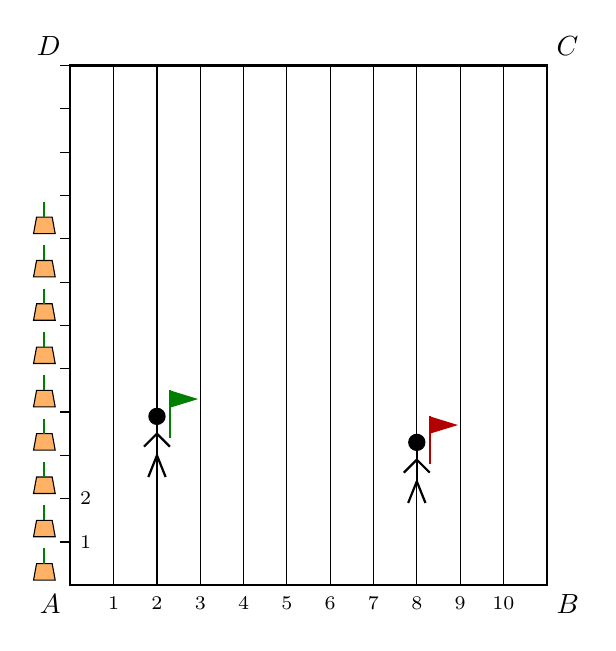
\begin{tikzpicture}[scale=0.55]
% the field: 11 m wide, drawn tall; the 10 chalk lines are 1 m apart
\draw[thick] (0,0) rectangle (11,12);
\foreach \x in {1,...,10}{\draw (\x,0)--(\x,12); \node[below,font=\scriptsize] at (\x,-0.05) {\x};}
% flower pots along AD (only the lower ones drawn), tick marks every metre
\foreach \i in {0,...,8}{%
  \draw[fill=orange!60] (-0.85,\i+0.12)--(-0.35,\i+0.12)--(-0.42,\i+0.5)--(-0.78,\i+0.5)--cycle;
  \draw[green!50!black,thick] (-0.6,\i+0.5)--(-0.6,\i+0.85);}
\foreach \i in {1,...,12}{\draw (-0.25,\i)--(0,\i);}
\node[right,font=\scriptsize] at (0,1) {1};
\node[right,font=\scriptsize] at (0,2) {2};
% the two runners with their flags (positions as in the question)
\begin{scope}[shift={(2,3)}]
 \draw[thick] (0,0)--(0,0.7); \draw[thick] (0,0)--(-0.2,-0.5); \draw[thick] (0,0)--(0.2,-0.5);
 \draw[thick] (0,0.5)--(0.3,0.2); \draw[thick] (0,0.5)--(-0.3,0.2); \fill (0,0.9) circle (0.2);
 \draw[green!50!black,thick] (0.3,0.4)--(0.3,1.5); \fill[green!50!black] (0.3,1.5)--(0.95,1.3)--(0.3,1.1)--cycle;
\end{scope}
\begin{scope}[shift={(8,2.4)}]
 \draw[thick] (0,0)--(0,0.7); \draw[thick] (0,0)--(-0.2,-0.5); \draw[thick] (0,0)--(0.2,-0.5);
 \draw[thick] (0,0.5)--(0.3,0.2); \draw[thick] (0,0.5)--(-0.3,0.2); \fill (0,0.9) circle (0.2);
 \draw[red!70!black,thick] (0.3,0.4)--(0.3,1.5); \fill[red!70!black] (0.3,1.5)--(0.95,1.3)--(0.3,1.1)--cycle;
\end{scope}
\node[below left] at (0,0) {$A$};\node[below right] at (11,0) {$B$};
\node[above right] at (11,12) {$C$};\node[above left] at (0,12) {$D$};
\end{tikzpicture}%
\figcap{Fig.\ 7.12 (redrawn, not to scale). Chalk lines numbered $1$ to $10$ from $A$ along $AB$; flower pots 1~m apart along $AD$ (only some are drawn); green flag on line 2, red flag on line 8.}
\end{center}

\textbf{Solution.}

\textbf{Step 1: length of $AD$.} 100 flower pots are placed 1~m apart along $AD$, so $AD=100$~m (this is the value the book intends).

\textbf{Step 2: set up coordinates.} Take $A$ as the origin, $AB$ along the $x$-axis and $AD$ along the $y$-axis, with 1 unit = 1~m. The chalk lines are 1~m apart and numbered from $A$, so the $n$th line is the line $x=n$. A flag on the $n$th line therefore has $x$-coordinate $n$, and its $y$-coordinate is its distance from $AB$ measured along the line.
\slip{``The 2nd line'' gives the $x$-coordinate ($x=2$), not the $y$-coordinate. The fraction of $AD$ gives the $y$-coordinate.}

\textbf{Step 3: position of each flag.}\\
Green flag: on the 2nd line, so $x=2$. Niharika runs $\frac14$ of $AD$, so $y=\frac14\times100=25$. So $G(2,25)$.\\
Red flag: on the 8th line, so $x=8$. Preet runs $\frac15$ of $AD$, so $y=\frac15\times100=20$. So $R(8,20)$.

\textbf{Step 4: distance between the flags.} By the distance formula $d=\sqrt{(x_2-x_1)^2+(y_2-y_1)^2}$ with $(x_1,y_1)=(2,25)$ and $(x_2,y_2)=(8,20)$:
\begin{align*}
\distn{GR}{2}{25}{8}{20}
\end{align*}
$\sqrt{61}\approx7.81$ and $61$ has no square factor, so it stays as $\sqrt{61}$.

\textbf{Step 5: the blue flag.} Rashmi posts it halfway between the two flags, that is at the mid-point of $GR$. By the mid-point formula $\left(\dfrac{x_1+x_2}{2},\dfrac{y_1+y_2}{2}\right)$:
\[
\left(\frac{2+8}{2},\ \frac{25+20}{2}\right)=\left(\frac{10}{2},\ \frac{45}{2}\right)=(5,\ 22.5).
\]

\textbf{Verification.} The blue flag $B_1(5,22.5)$ should be equally far from both flags. Using $d^2=(x_2-x_1)^2+(y_2-y_1)^2$:
\begin{align*}
B_1G^2&=(2-5)^2+(25-22.5)^2=(-3)^2+(2.5)^2=9+6.25=15.25\\
B_1R^2&=(8-5)^2+(20-22.5)^2=3^2+(-2.5)^2=9+6.25=15.25
\end{align*}
Each is $15.25=\dfrac{61}{4}$, so each distance is $\dfrac{\sqrt{61}}{2}$, which is half of $GR$.

\ans{The distance between the two flags is $\sqrt{61}$ m ($\approx7.81$ m). Rashmi should post the blue flag at $(5,22.5)$, that is on the 5th line, $22.5$ m from $AB$ along that line.}

%---------------------------------------------------------------
\subsection*{Exercise 7.2, Question 4}
\textbf{Question.} Find the ratio in which the line segment joining the points $(-3,10)$ and $(6,-8)$ is divided by $(-1,6)$.

\textbf{Solution.} Let $A(-3,10)$, $B(6,-8)$ and let $P(-1,6)$ divide $AB$ in the ratio $m_1:m_2$. So $(x_1,y_1)=(-3,10)$ and $(x_2,y_2)=(6,-8)$.

By the section formula, $x=\dfrac{m_1x_2+m_2x_1}{m_1+m_2}$:
\begin{align*}
-1&=\frac{m_1(6)+m_2(-3)}{m_1+m_2}=\frac{6m_1-3m_2}{m_1+m_2}\\
-(m_1+m_2)&=6m_1-3m_2\\
-m_1-m_2&=6m_1-3m_2\\
3m_2-m_2&=6m_1+m_1\\
2m_2&=7m_1\\
\frac{m_1}{m_2}&=\frac27
\end{align*}
So the ratio is $2:7$.

\textbf{Check with the $y$-coordinate.} Put $m_1=2$, $m_2=7$ in $y=\dfrac{m_1y_2+m_2y_1}{m_1+m_2}$:
\[\frac{2(-8)+7(10)}{2+7}=\frac{-16+70}{9}=\frac{54}{9}=6,\]
which is the $y$-coordinate of $P$. The ratio is correct.

\ans{The ratio is $2:7$.}

%---------------------------------------------------------------
\subsection*{Exercise 7.2, Question 5}
\textbf{Question.} Find the ratio in which the line segment joining $A(1,-5)$ and $B(-4,5)$ is divided by the $x$-axis. Also find the coordinates of the point of division.

\textbf{Solution.} Let the $x$-axis divide $AB$ at $P$ in the ratio $k:1$. A point on the $x$-axis has $y$-coordinate $0$. Here $(x_1,y_1)=(1,-5)$, $(x_2,y_2)=(-4,5)$, $m_1=k$, $m_2=1$.

By the section formula $\left(\dfrac{m_1x_2+m_2x_1}{m_1+m_2},\dfrac{m_1y_2+m_2y_1}{m_1+m_2}\right)$:
\[
P=\left(\frac{k(-4)+1(1)}{k+1},\ \frac{k(5)+1(-5)}{k+1}\right)=\left(\frac{1-4k}{k+1},\ \frac{5k-5}{k+1}\right).
\]
The $y$-coordinate of $P$ is $0$:
\[\frac{5k-5}{k+1}=0\ \Rightarrow\ 5k-5=0\ \Rightarrow\ k=1 .\]
So the ratio is $1:1$. Put $k=1$ in the $x$-coordinate:
\[x=\frac{1-4(1)}{1+1}=\frac{-3}{2}=-\frac32 .\]

\textbf{Verification.} A ratio $1:1$ means $P$ is the mid-point. By the mid-point formula,
\[
\left(\dfrac{x_1+x_2}{2},\dfrac{y_1+y_2}{2}\right)
\]
the mid-point of $AB$ is
\[
\left(\dfrac{1+(-4)}{2},\dfrac{-5+5}{2}\right)=\left(-\dfrac32,0\right),
\]
which lies on the $x$-axis.

\ans{The $x$-axis divides $AB$ in the ratio $1:1$ (at its mid-point), and the point of division is $\left(-\dfrac32,0\right)$.}

%---------------------------------------------------------------
\subsection*{Exercise 7.2, Question 6}
\textbf{Question.} If $(1,2)$, $(4,y)$, $(x,6)$ and $(3,5)$ are the vertices of a parallelogram taken in order, find $x$ and $y$.

\textbf{Solution.} Let $A(1,2)$, $B(4,y)$, $C(x,6)$, $D(3,5)$. The diagonals of a parallelogram bisect each other, so the mid-points of the diagonals $AC$ and $BD$ coincide.

By the mid-point formula $\left(\dfrac{x_1+x_2}{2},\dfrac{y_1+y_2}{2}\right)$:
\[
\begin{gathered}
\text{Mid-point of }AC=\left(\frac{1+x}{2},\frac{2+6}{2}\right)=\left(\frac{1+x}{2},4\right),\\
\text{Mid-point of }BD=\left(\frac{4+3}{2},\frac{y+5}{2}\right)=\left(\frac72,\frac{y+5}{2}\right).
\end{gathered}
\]
Equate the $x$-coordinates and the $y$-coordinates:
\[
\frac{1+x}{2}=\frac72\ \Rightarrow\ 1+x=7\ \Rightarrow\ x=6,\qquad 4=\frac{y+5}{2}\ \Rightarrow\ y+5=8\ \Rightarrow\ y=3 .
\]

\textbf{Verification.} With $A(1,2)$, $B(4,3)$, $C(6,6)$, $D(3,5)$, opposite sides should be equal. By $d^2=(x_2-x_1)^2+(y_2-y_1)^2$:
\begin{align*}
AB^2&=(4-1)^2+(3-2)^2=3^2+1^2=9+1=10\\
DC^2&=(6-3)^2+(6-5)^2=3^2+1^2=9+1=10\\
BC^2&=(6-4)^2+(6-3)^2=2^2+3^2=4+9=13\\
AD^2&=(3-1)^2+(5-2)^2=2^2+3^2=4+9=13
\end{align*}
So $AB=DC$ and $BC=AD$: opposite sides are equal.

\ans{$x=6$ and $y=3$.}

%---------------------------------------------------------------
\subsection*{Exercise 7.2, Question 7}
\textbf{Question.} Find the coordinates of a point $A$, where $AB$ is the diameter of a circle whose centre is $(2,-3)$ and $B$ is $(1,4)$.

\textbf{Solution.} The centre of a circle is the mid-point of every diameter. Let $A(x,y)$ and $B(1,4)$; the centre $(2,-3)$ is the mid-point of $AB$.

By the mid-point formula $\left(\dfrac{x_1+x_2}{2},\dfrac{y_1+y_2}{2}\right)$:
\[
\frac{x+1}{2}=2\ \Rightarrow\ x+1=4\ \Rightarrow\ x=3,\qquad \frac{y+4}{2}=-3\ \Rightarrow\ y+4=-6\ \Rightarrow\ y=-10 .
\]

\textbf{Verification.} The mid-point of $A(3,-10)$ and $B(1,4)$ is $\left(\dfrac{3+1}{2},\dfrac{-10+4}{2}\right)=\left(\dfrac42,\dfrac{-6}{2}\right)=(2,-3)$, the given centre.

\ans{$A$ is $(3,-10)$.}

%---------------------------------------------------------------
\subsection*{Exercise 7.2, Question 8}
\textbf{Question.} If $A$ and $B$ are $(-2,-2)$ and $(2,-4)$, respectively, find the coordinates of $P$ such that $AP=\dfrac37AB$ and $P$ lies on the line segment $AB$.

\textbf{Solution.} Since $P$ lies on segment $AB$, $PB=AB-AP=AB-\frac37AB=\frac47AB$.
Therefore $AP:PB=\frac37AB:\frac47AB=3:4$.

By the section formula $\left(\dfrac{m_1x_2+m_2x_1}{m_1+m_2},\dfrac{m_1y_2+m_2y_1}{m_1+m_2}\right)$ with $A(-2,-2)$, $B(2,-4)$ and $m_1:m_2=3:4$:
\begin{align*}
x&=\frac{3(2)+4(-2)}{3+4}=\frac{6-8}{7}=-\frac27\\
y&=\frac{3(-4)+4(-2)}{3+4}=\frac{-12-8}{7}=-\frac{20}{7}
\end{align*}
\slip{$AP=\frac37AB$ does not mean the ratio is $3:7$. The ratio $AP:PB$ is $3:4$, because $PB=AB-AP=\frac47AB$.}

\textbf{Verification.} By the distance formula $d=\sqrt{(x_2-x_1)^2+(y_2-y_1)^2}$:
\begin{align*}
AB&=\sqrt{(2-(-2))^2+(-4-(-2))^2}=\sqrt{4^2+(-2)^2}=\sqrt{16+4}=\sqrt{20}=2\sqrt5\\
AP&=\sqrt{\left(-\tfrac27-(-2)\right)^2+\left(-\tfrac{20}{7}-(-2)\right)^2}=\sqrt{\left(\tfrac{12}{7}\right)^2+\left(-\tfrac67\right)^2}=\sqrt{\tfrac{144}{49}+\tfrac{36}{49}}=\sqrt{\tfrac{180}{49}}=\tfrac{6\sqrt5}{7}
\end{align*}
and $\frac37AB=\frac37\times2\sqrt5=\frac{6\sqrt5}{7}=AP$.

\ans{$P\left(-\dfrac27,-\dfrac{20}{7}\right)$.}

%---------------------------------------------------------------
\subsection*{Exercise 7.2, Question 9}
\textbf{Question.} Find the coordinates of the points which divide the line segment joining $A(-2,2)$ and $B(2,8)$ into four equal parts.

\textbf{Solution.} Let $P$, $Q$, $R$ be the points that divide $AB$ into four equal parts, in order from $A$. Then $P$ divides $AB$ in the ratio $1:3$, $Q$ is the mid-point of $AB$ (ratio $2:2=1:1$), and $R$ divides $AB$ in the ratio $3:1$. Here $(x_1,y_1)=(-2,2)$ and $(x_2,y_2)=(2,8)$.

By the section formula $\left(\dfrac{m_1x_2+m_2x_1}{m_1+m_2},\dfrac{m_1y_2+m_2y_1}{m_1+m_2}\right)$:

$P$ ($m_1:m_2=1:3$): $x=\dfrac{1(2)+3(-2)}{1+3}=\dfrac{2-6}{4}=-1$, $y=\dfrac{1(8)+3(2)}{1+3}=\dfrac{8+6}{4}=\dfrac{14}{4}=\dfrac72$.

$Q$ (mid-point formula $\left(\dfrac{x_1+x_2}{2},\dfrac{y_1+y_2}{2}\right)$): $x=\dfrac{-2+2}{2}=0$, $y=\dfrac{2+8}{2}=5$.

$R$ ($m_1:m_2=3:1$): $x=\dfrac{3(2)+1(-2)}{3+1}=\dfrac{6-2}{4}=1$, $y=\dfrac{3(8)+1(2)}{3+1}=\dfrac{24+2}{4}=\dfrac{26}{4}=\dfrac{13}{2}$.

\textbf{Verification.} $Q$ should be the mid-point of $PR$: $\left(\dfrac{-1+1}{2},\dfrac{\frac72+\frac{13}{2}}{2}\right)=\left(0,\dfrac{10}{2}\right)=(0,5)=Q$.

\ans{The points are $P\left(-1,\dfrac72\right)$, $Q(0,5)$ and $R\left(1,\dfrac{13}{2}\right)$.}

%---------------------------------------------------------------
\subsection*{Exercise 7.2, Question 10}
\textbf{Question.} Find the area of a rhombus if its vertices are $(3,0)$, $(4,5)$, $(-1,4)$ and $(-2,-1)$ taken in order. [Hint: Area of a rhombus $=\frac12$ (product of its diagonals)]

\textbf{Solution.} Let $A(3,0)$, $B(4,5)$, $C(-1,4)$, $D(-2,-1)$. The diagonals are $AC$ and $BD$. By the distance formula $d=\sqrt{(x_2-x_1)^2+(y_2-y_1)^2}$:

\distnote
\begin{align*}
\dist{AC}{3}{0}{-1}{4}{4\sqrt2}\\
\dist{BD}{4}{5}{-2}{-1}{6\sqrt2}
\end{align*}
(Here $\sqrt{32}=\sqrt{16\times2}=4\sqrt2$ and $\sqrt{72}=\sqrt{36\times2}=6\sqrt2$.)

By the hint, $\text{Area}=\dfrac12\,d_1d_2$ with $d_1=4\sqrt2$ and $d_2=6\sqrt2$:
\[
\text{Area}=\frac12\times4\sqrt2\times6\sqrt2=\frac12\times(4\times6)\times(\sqrt2\times\sqrt2)=\frac12\times24\times2=24 .
\]
\slip{The area is $\frac12d_1d_2$, not $d_1d_2$. Do not forget the $\frac12$.}

\textbf{Verification that $ABCD$ is a rhombus.} All four sides should be equal:
\begin{align*}
\distn{AB}{3}{0}{4}{5}\\
\distn{BC}{4}{5}{-1}{4}\\
\distn{CD}{-1}{4}{-2}{-1}\\
\distn{DA}{-2}{-1}{3}{0}
\end{align*}
All four sides are $\sqrt{26}$, so the quadrilateral is a rhombus and the hint applies.

\ans{The area of the rhombus is $24$ square units.}
